\documentclass[12pt,fleqn]{beamer}
%\usepackage{verbatim}
%\usetheme[]{Singapore}
%\usetheme[]{Antibes}
%\usetheme[]{Warsaw}

%\setbeamercolor{structure}{blue}
%\setbeamercolor{structure}{black}
%\setbeamercolor{structure}{white}


%\beamertemplategridbackground[12.0pt]
%\beamertemplateshadingbackground{black}{black}
%\beamertemplateshadingbackground{blue!65}{black}
%\beamertemplateshadingbackground{blue!45}{blue!45}
\beamertemplateshadingbackground{black!10}{black!30}


%\beamertemplateshadingbackground{black}{black}

\usepackage{amsmath,amssymb,dsfont,mathrsfs}
%\usepackage{amsmath,amssymb}
\usepackage{tikz,pgflibraryplotmarks}
%\usepackage{multimedia}
\usepackage{wasysym}
\usepackage{rotating}
%\usepackage{movie15}



\xdefinecolor{lavendar}{rgb}{0.8,0.6,1}
\xdefinecolor{olive}{cmyk}{0.64,0,0.95,0.4}
%\xdefinecolor{olive}{cmyk}{1,0,0,0}
\xdefinecolor{mag}{cmyk}{0.1,1,0,0.2}
\xdefinecolor{lblue}{rgb}{0,0,1.5}
\xdefinecolor{lred}{rgb}{1,0,0}
\xdefinecolor{mine}{cmyk}{1,0,0.2,0}
\xdefinecolor{bluel}{cmyk}{0.1,0,0.9,0.4}



%\newcommand{\tcr}{\textcolor{white}}
\newcommand{\tcr}{\textcolor{red}}
%\newcommand{\tcr}{\textcolor{yellow}}
%\newcommand{\tcrd}{\textcolor{yellow}}
\newcommand{\tcrd}{\textcolor{red}}


%\newcommand{\tcr}{\textcolor{lred}}
%\newcommand{\tcw}{\textcolor{gray}}
\newcommand{\tcw}{\textcolor{white}}
%\newcommand{\tcw}{\textcolor{black}}

%\newcommand{\tcw}{\textcolor{black}}

%\newcommand{\tcb}{\textcolor{blue}}
\newcommand{\tcb}{\textcolor{bluel}}
\newcommand{\tcm}{\textcolor{mag}}
\newcommand{\tcg}{\textcolor{olive}}

\newcommand{\bfC}{\bf C}
\newcommand{\dC}{\bf C_{u}}
\newcommand{\hf}{\frac 12}

\newcommand{\E}{\vec E}
\newcommand{\vu}{  {\vec {\bf u}}}
\newcommand{\ve}{  {\vec {\bf e}}}

\newcommand{\bfu}{  { {\bf u}}}

\newcommand{\grad}{  {\vec {\bf \nabla}}}


\newcommand{\lfrownie}{\textcolor{red}{\large{\frownie}}}
\newcommand{\lsmiley}{\textcolor{green}{\large{\smiley}}}

\newcommand{\curl}{\ensuremath{\nabla\times\,}}
\renewcommand{\div}{\nabla\cdot\,}
\newcommand{\divh}{\nabla_h\cdot\,}
\renewcommand{\grad}{\ensuremath{\nabla}}
\newcommand\makebeamertitle{\frame{\maketitle}}%




\title{Computational Methods for Engineers}
\subtitle{how to waste  your time on writing code and have lots of fun }

\author[Haber ]{Eldad Haber } 
\institute{
  
}


\date{Jan 2020}




\begin{document}

\makebeamertitle




\section{Introduction} % (fold)
\label{sec:introduction}

\begin{frame}\frametitle{Outline}
\begin{itemize}
	\item Goals of this course
	\item Integrating math/physics/code
	\item Python
	\item Your commitment 
\end{itemize}
\end{frame}

\begin{frame}
	\frametitle{Scientific Computing}
	aka: Computational Science, Scientific Computation
	
	\begin{itemize}
		\item Simulations
		\item Data fitting and analysis
		\item Optimization
		\item Visualization
		\item \ldots
	\end{itemize}
	
	Goal: Gain understanding through analysis of mathematical models implemented on computers.
	
\end{frame}

\begin{frame}
	\frametitle{Steps in Computational Science}
	
\begin{itemize}
\item A story - observation
\item Mathematical model
\item Discretization of the model
\item Solving the model 
\item Parameters fitting
\item Visualizing the result
\end{itemize}	

\end{frame}


\begin{frame}
	\frametitle{Example I: Newton's apple}
	
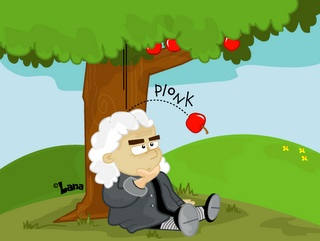
\includegraphics[width=2.5cm]{apple-newton}
\begin{itemize}
\item Observation - Apple is falling
\item Math model 
$${\frac {d^{2}x}{dt^{2}}} = -g$$ (but what is $g$?)
\item Discretization
$$ {\frac {x(t_{i+1}) - 2 x(t_{i}) + x(t_{i-1})}{\Delta t^{2}}} = -g. $$
\item Solve
$$	x(t_{i+1}) = -g \Delta t^{2} + 2 x(t_{i}) - x(t_{i-1}) $$
\item Measure and find an approximation to $g$
\item Visualize
\end{itemize}
	
	
\end{frame}


\begin{frame}
\frametitle{Example I:  Newton's apple}

{\bf Data assimilation}

What is $g$?

\vspace{12pt}

Observations (noisy)
$$ t = [0,\ 1,\ 2,\ 3] \quad \quad x = [0,\ 4.4,\  21.0,\ 54.2] $$

\begin{itemize}
\item Can the mathematical model (reasonably) explain the data?
\item What is the (best) value of $g$?
\end{itemize}


\end{frame}


\begin{frame}
\frametitle{Example II: Ground water flow}

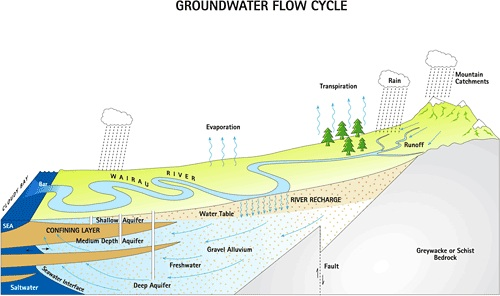
\includegraphics[width=3.5cm]{GroundwaterFlowCycle}
\begin{itemize}
\item Observation - Water flow in the ground
\item Math model 
$$\nabla \cdot \sigma \nabla p = q\quad \quad \rho_{t} + \div (\sigma \nabla p ) \rho = 0$$
\item Discretization ... (you will know all about this)
\item Solve ... (you will know all about this)
\item Visualize
\end{itemize}

\end{frame}

\begin{frame}
\frametitle{Example III: Pattern identification}

Simplest example - Character recognition.
We have digits ([0,...,9]) in an image and we want to get them explicitly.

\begin{center}
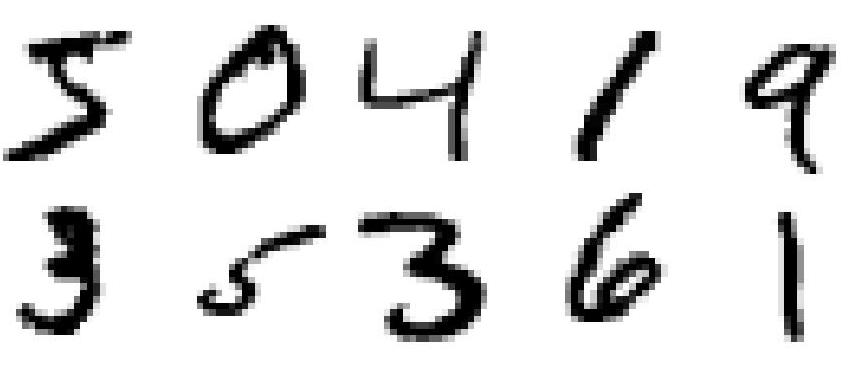
\includegraphics[width=8cm]{digits.jpg}
\end{center}

\vspace{1cm}

Mathematical model - ???

\end{frame}

\begin{frame}
\frametitle{Example III: Pattern identification}



Machine learning, try the following model known as Convolution Neural Network 
$$ {\bf y} = {\bf w}^{\top} {\rm tanh}( \bf K \star {\bf x} + {\bf b} ) $$

\vspace{1cm}

No physical basis so we hope it can do the trick ...


\end{frame}

\begin{frame}
\frametitle{Example III: Pattern identification}

$$ {\bf y} = {\bf w}^{\top} {\rm tanh}( \bf K \star {\bf x} + {\bf b} ) $$

\begin{itemize}
\item $\bf y$ vector of $10$, with probabilities of the digits\\
Example: $ [0,0.65,0,0,0,0,0,0.35,0,0] $ imply $65\%$ the number $1$ and
$35\%$ the number $7$
\item $\bf x$ the image
\item $\bf K$, $\bf b$ and $\bf w$ parameters
\end{itemize}

\end{frame}


\begin{frame}
\frametitle{Example III: Pattern identification}

Pattern recognition can be applied for
many problems when the math is too complex
or unknown
\begin{itemize}
\item Climate prediction
\item Weather
\item Flow in complex systems
\item Much more ...
\end{itemize}




\end{frame}


\begin{frame}
\frametitle{Goal of this course}

\begin{itemize}
\item Describe useful physical models in earth science
\begin{enumerate}
\item Flow in porous media
\item Pressure system
\item Heat propagation
\end{enumerate}
\item Learn how to simulate them on the computer
\item Learn how to integrate field data into physical models
\end{itemize}

\end{frame}

\begin{frame}
\frametitle{Integration of Physics/Math/Computing}

This course has a new paradigm. We 
\begin{itemize}
\item Describe the physics
\item Develop a mathematical model
\item Write code to simulate this model
\end{itemize}

\vspace{12pt}

We will cover most of the math you need but we will use
\begin{itemize}
\item Vector calculus
\item Differential equations
\item Linear algebra
\item Python programming
\end{itemize}


\end{frame}


\begin{frame}
\frametitle{Computing}

\begin{itemize}
\item The course will involve {\bf lots} of programming and computing
\item Bring your laptop
\item Code will be handled through GitHub
\item Working in groups, encouraged!
\end{itemize}

\end{frame}

\begin{frame}
\frametitle{Python}

\begin{itemize}
\item We will be coding with Python and use Jupyter Notebooks
\item Main packages we use: NumPy and Torch.
\item Tutorials on Python and using NumPy and PyTorch can be found at \\
{\tt http://cs231n.github.io/python-numpy-tutorial/} \\
{\tt https://pytorch.org/tutorials/}
\end{itemize}

\end{frame}


\begin{frame}
\frametitle{Grading}

\begin{itemize}
\item Homework and programming assignments $40\%$
\item Midterms $30\%$
\item Final $30\%$ 
\end{itemize}

{\bf You need a pass in the final and homework to pass the course}



\end{frame}




\end{document}


